% Hình: Minh hoạ bài toán phân đoạn ảnh y sinh (Mục 3.1)
% Gói: TikZ thuần + \includegraphics (ảnh thật PH2 & GlaS)
\documentclass[border=6pt]{standalone}
\usepackage[utf8]{vietnam}
\usepackage{amsmath,amssymb}
\usepackage{graphicx}
\usepackage{xcolor}
\usepackage{tikz}
\usetikzlibrary{positioning,fit,arrows.meta,calc,backgrounds}
% ---- Bảng màu học thuật dùng chung ----
\definecolor{cvblue}{HTML}{35618E}
\definecolor{decgreen}{HTML}{5E7F4E}
\definecolor{qpurple}{HTML}{7E57C2}
\definecolor{lssorange}{HTML}{CF8A2A}
\definecolor{slate}{HTML}{5B6470}
\definecolor{inkdark}{HTML}{23272E}
\tikzset{
  >={Stealth[length=2.4mm]},
  every node/.style={font=\sffamily\small, text=inkdark},
  frame/.style={draw=slate, line width=0.8pt, inner sep=0pt},
  lbl/.style={font=\sffamily\footnotesize, text=slate},
  flow/.style={-{Stealth[length=2.6mm]}, line width=1pt, draw=inkdark},
}
\begin{document}
\begin{tikzpicture}[node distance=6mm]
  % --- Hàng PH2 ---
  \node[frame] (ph2img) {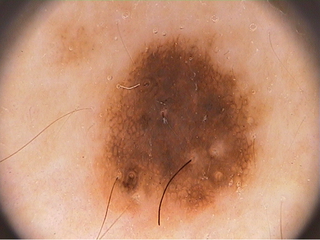
\includegraphics[width=3.1cm]{ph2_image.png}};
  \node[frame, right=16mm of ph2img] (ph2msk) {
\includegraphics[width=3.1cm]{ph2_mask.png}};
  \draw[flow] (ph2img) -- node[above, lbl] {$f_\theta$} (ph2msk);
  \node[lbl, below=1mm of ph2img] {Ảnh gốc $X\in\mathbb{R}^{H\times W\times 3}$};
  \node[lbl, below=1mm of ph2msk] {Mặt nạ $Y\in\{0,1\}^{H\times W}$};
  \node[left=3mm of ph2img, rotate=90, font=\sffamily\small\bfseries, text=cvblue] {PH2};

  % --- Hàng GlaS ---
  \node[frame, below=16mm of ph2img] (glimg) {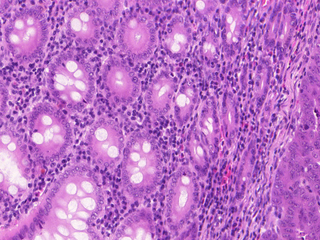
\includegraphics[width=3.1cm]{glas_image.png}};
  \node[frame, right=16mm of glimg] (glmsk) {
\includegraphics[width=3.1cm]{glas_mask.png}};
  \draw[flow] (glimg) -- node[above, lbl] {$f_\theta$} (glmsk);
  \node[lbl, below=1mm of glimg] {Ảnh mô học H\&E};
  \node[lbl, below=1mm of glmsk] {Mặt nạ vùng tuyến};
  \node[left=3mm of glimg, rotate=90, font=\sffamily\small\bfseries, text=decgreen] {GlaS};
\end{tikzpicture}
\end{document}
